% Version 1.0   Aug  4, 2020   by GJ Woeginger
% Version 2.0   Aug 13, 2020   by GJ Woeginger
% Version 2.1   Aug 17, 2020   by GJ Woeginger
% Version 2.2   Sep  1, 2020   by GJ Woeginger

\documentclass[11pt,fleqn]{article}

\usepackage{amsmath,amssymb,graphicx}

\usepackage{tikz,tikzsymbols}
\usetikzlibrary{shapes,patterns,positioning}
\usetikzlibrary{arrows,decorations.markings}
\usetikzlibrary{calc}

\textheight=21.20truecm
\textwidth=14.70truecm
\hoffset=-1.20truecm
\voffset=-1.10truecm

\begin{document}
\sloppy
\newtheorem{axiom}{Axiom}[section]
\newtheorem{conjecture}[axiom]{Conjecture}
\newtheorem{corollary}[axiom]{Corollary}
\newtheorem{definition}[axiom]{Definition}
\newtheorem{example}[axiom]{Example}
\newtheorem{fact}[axiom]{Fact}
\newtheorem{lemma}[axiom]{Lemma}
\newtheorem{observation}[axiom]{Observation}
\newtheorem{proposition}[axiom]{Proposition}
\newtheorem{theorem}[axiom]{Theorem}

\renewcommand{\topfraction}{1.0}
\renewcommand{\bottomfraction}{1.0}

%%%%%%%%%%%%%%%%%%%%%%%%%%%%%%%%%%%%%%%%%%%%%%
%%  GJW: macros
%%%%%%%%%%%%%%%%%%%%%%%%%%%%%%%%%%%%%%%%%%%%%%
\newcommand{\proof}{\emph{Proof.}\ \ }
\newcommand{\qed}{~~$\Box$}
\newcommand{\RRR}{{\mathbb{R}_{\ge0}}}

\newcommand{\spp}{\text{SPP}}
\newcommand{\qspp}{\text{QSPP}}
\newcommand{\ppp}{{\cal P}_{st}}
\newcommand{\pppx}{{\cal P}^+}
\newcommand{\pppy}{{\cal P}^-}

\newcommand{\boxxx}[1]
 {\fbox{\begin{minipage}{13.00cm}\begin{center}\bigskip\begin{minipage}{12.30cm}
  #1\end{minipage}\end{center}~\end{minipage}}}


%%%%%%%%%%%%%%%%%%%%%%%%%%%%%%%%%%%%%%%%%%%%%%%%%%%%%%%%%%%%%%%%%%%%%%%%%%
%%%%%%%%%%%%%%%%%%%%%%%%%%%%%%%%%%%%%%%%%%%%%%%%%%%%%%%%%%%%%%%%%%%%%%%%%%
\title{{\bf Linearizable special cases of\\the quadratic shortest path problem}}
\author{
\sc Eranda \c{C}ela\thanks{{\tt cela@math.tugraz.at}.
Institute of Discrete Mathematics, TU Graz, Austria.}
\and
\sc ~~Bettina Klinz\thanks{{\tt klinz@opt.math.tugraz.at}.
Institute of Discrete Mathematics, TU Graz, Austria.}
\and
\sc ~Stefan Lendl\thanks{{\tt lendl@math.tugraz.at}.
Institute of Discrete Mathematics, TU Graz, Austria.}
\and
\sc James B. Orlin\thanks{{\tt jorlin@mit.edu}.
Sloan School of Management, M.I.T., Cambridge, USA.}
\and
\sc Gerhard J. Woeginger\thanks{{\tt woeginger@algo.rwth-aachen.de}.
Department of Computer Science, RWTH Aachen, Germany.}
\and
\sc Lasse Wulf\thanks{{\tt wulf@math.tugraz.at}.
Institute of Discrete Mathematics, TU Graz, Austria.}
}
\date{}
\maketitle

\begin{abstract}
The quadratic shortest path problem (QSPP) in a directed graph asks for a directed path 
from a given source vertex to a given sink vertex, so that the sum of the interaction 
costs over all pairs of arcs on the path is minimized.
We consider special cases of the QSPP that are linearizable as a shortest path problem
in the sense of Bookhold.
If the QSPP on a directed graph is linearizable under all possible choices of the arc 
interaction costs, the graph is called universally linearizable.

We provide various combinatorial characterizations of universally linearizable graphs that 
are centered around the structure of source-to-sink paths and around certain forbidden subgraphs.
Our characterizations lead to fast and simple recognition algorithms for universally 
linearizable graphs.
Furthermore, we establish the intractability of deciding whether a concrete instance of 
the QSPP (with a given graph and given arc interaction costs) is linearizable.

\bigskip\noindent\emph{Keywords:}
discrete optimization; shortest path problem; computational complexity.
\end{abstract}

\newpage
%%%%%%%%%%%%%%%%%%%%%%%%%%%%%%%%%%%%%%%%%%%%%%%%%%%%%%%%%%%%%%%%%%%%%%%%%
%%%%%%%%%%%%%%%%%%%%%%%%%%%%%%%%%%%%%%%%%%%%%%%%%%%%%%%%%%%%%%%%%%%%%%%%%
\section{Introduction}
%%%%%%%%%%%%%%%%%%%%%%%%%%%%%%%%%%%%%%%%%%%%%%%%%%%%%%%%%%%%%%%%%%%%%%%%
The \emph{Shortest Path Problem} (SPP) is a well-known and fundamental problem in 
combinatorial optimization; see for instance Schrijver \cite{Schrijver2012}.
An instance of SPP consists of a directed graph $G=(V,A)$ together with a source vertex $s\in V$, 
a sink vertex $t\in V$, and weights $w(a)\in\RRR$ for the arcs $a\in A$.
For a simple directed $s$-$t$-path~$P$ that traverses the arcs $a_1,a_2,\ldots,a_p$ in that order,
its \emph{SPP-weight} is given by
%%%%%%%%%%%%%%%%
\begin{equation}
\label{eq:SPP}
\spp(P,w) ~:=~ \sum_{i=1}^p~ w(a_i).
\end{equation}
%%%%%%%%%%%%%%%%
The \emph{Quadratic Shortest Path Problem} (QSPP) takes as input a directed graph $G=(V,A)$ together
with a source $s\in V$ and a sink $t\in V$.
Every pair of arcs $a,a'\in A$ comes with an interaction cost $q(a,a')\in\RRR$;
we assume throughout that $q(a,a')=q(a',a)$ holds for all $a,a'\in A$.
For a simple directed $s$-$t$-path $P$ that traverses the arcs $a_1,a_2,\ldots,a_p$ in that order,
its \emph{QSPP-cost} is given by 
%%%%%%%%%%%%%%%%
\begin{equation}
\label{eq:QSPP}
\qspp(P,q) ~:=~ \sum_{i=1}^p\sum_{j=1}^p~ q(a_i,a_j).
\end{equation}
%%%%%%%%%%%%%%%%
The goal in the SPP and in the QSPP is to determine a simple directed $s$-$t$-path $P$ that 
minimizes the respective objective values (\ref{eq:SPP}) and (\ref{eq:QSPP}).
The SPP is polynomially solvable; see for instance Cormen, Leiserson, Rivest \& Stein \cite{CLRS}.
The QSPP is NP-hard and extremely difficult to solve;
see for instance Rostami, Malucelli, Frey~\& Buchheim~\cite{Rostami-1},
Rostami \& al~\cite{Rostami-2}, and Hu \& Sotirov~\cite{HuSo2018a,HuSo2018b,HuSo2020}.

%%%%%%%%%%%%%%%%%%%%%%%%%%%%%%%%%%%%%%%%%
\begin{figure}[b]
\hrule\hrule
\medskip
\bigskip
\begin{center}
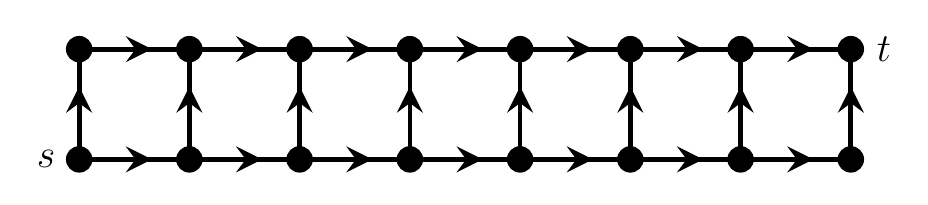
\begin{tikzpicture}[scale=1.40]

\foreach \x in {1,...,8}
  {\fill (\x,0) circle (0.12);
   \fill (\x,1) circle (0.12);}

\node at ( 0.70, 0.00) {\Large$s$};
\node at ( 8.30, 1.00) {\Large$t$};

\foreach \x in {1,...,8}
{\draw[decoration={markings,mark=at position 0.66 with {\arrow[scale=1.5,>=stealth]{>}}},
    postaction={decorate},line width=1.70pt] (\x,0)--(\x,1);}

\foreach \x in {1,...,7}
{\draw[decoration={markings,mark=at position 0.66 with {\arrow[scale=1.5,>=stealth]{>}}},
    postaction={decorate},line width=1.70pt] (\x,0)--(\x+1,0);
 \draw[decoration={markings,mark=at position 0.66 with {\arrow[scale=1.5,>=stealth]{>}}},
    postaction={decorate},line width=1.70pt] (\x,1)--(\x+1,1);}

\end{tikzpicture}
\end{center}
\caption{The grid $G_{2,n}$ consists of two horizontal layers with $n$ vertices.
All horizontal arcs are oriented from west to east, and all vertical arcs are oriented from south to north.}
\label{fig:grid}
\bigskip
\hrule\hrule
\end{figure}
%%%%%%%%%%%%%%%%%%%%%%%%%%%%%%%%%%%%%%%%%

\paragraph{Linearizations.}
An instance of the QSPP is called \emph{linearizable}, if there exist arc weights $w:A\to\RRR$
for the SPP on the same directed graph $G$ such that
%%%%%%%%%%%%%%%%
\begin{equation}
\label{eq:linearizable}
\qspp(P,q) = \spp(P,w) \text{\qquad\quad for all simple directed $s$-$t$-paths $P$.}
\end{equation}
%%%%%%%%%%%%%%%%
If we manage to find a linearization of a QSPP instance, we can of course solve the QSPP instance
by simply solving the linearized instance of the SPP instead.
Hu \& Sotirov \cite{HuSo2018a,HuSo2018b} were the first to study linearizations of the QSPP.
Among other results, they show in \cite{HuSo2018b} that for an \emph{acyclic} directed graph $G$
with given arc interaction costs, linearizability of the instance can be decided in polynomial time.
Furthermore \cite{HuSo2018a} proves that on the grid $G_{2,n}$ the QSPP is \emph{always} linearizable,
independently of the concrete arc interaction costs in the instance;
see Figure~\ref{fig:grid} for an illustration.

Linearizations of non-linear problems form a widely used standard tool in continuous 
optimization and numerical analysis.
On the discrete side, the linearization of hard combinatorial optimization problems by easy 
combinatorial optimization problems goes back to the seminal work of Bookhold \cite{Bo1990}, 
who linearized the NP-hard Quadratic Assignment Problem (QAP) via the polynomially solvable 
linear assignment problem.
Kabadi \& Punnen \cite{KaPu2011,PuKa2013} gave a polynomial time algorithm for recognizing 
linearizable instances of the QAP in Koopmans-Beckmann form.
Furthermore, \cite{PuKa2013} presented a purely combinatorial characterization of all linearizable
QAP instances with symmetric cost matrices.
Further results on linearizations of the QAP have been derived by
Erdo\u{g}an \cite{Erdogan2006}, Erdo\u{g}an \& Tansel \cite{ErTa2007,ErTa2011}, and 
\c{C}ela, Deineko \& Woeginger \cite{CeDeWo2016}.
{\'C}usti{\'c} \& Punnen \cite{CuPu2016} investigate linearizable instances of the quadratic minimum spanning tree problem,
Punnen, Walter \& Woods \cite{PuWaWo2013} study linearizable instances of the quadratic travelling salesman problem, and
De Meijer \& Sotirov \cite{deMeSo2020} analyze linearizations of the quadratic cycle cover problem.

%%%%%%%%%%%%%%%%%%%%%%%%%%%%%%%%%%%%%%%%%
\begin{figure}[bth]
\hrule\hrule
\medskip
\begin{center}
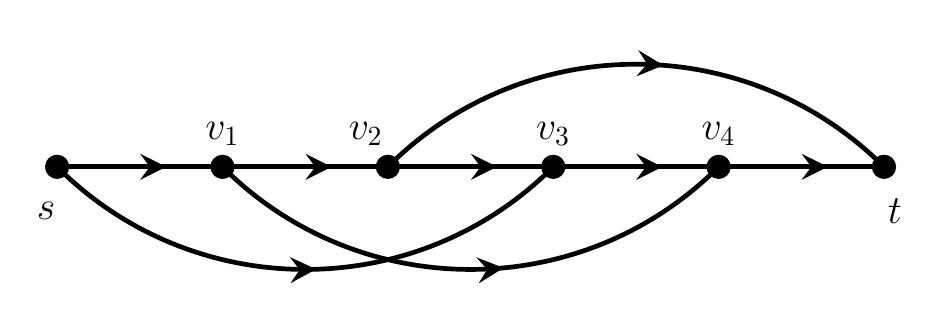
\begin{tikzpicture}[scale=1.40]

\coordinate (p0) at ( 0.0,0);
\coordinate (p1) at ( 1.5,0);
\coordinate (p2) at ( 3.0,0);
\coordinate (p3) at ( 4.5,0);
\coordinate (p4) at ( 6.0,0);
\coordinate (p5) at ( 7.5,0);

\foreach \x in {0,...,5}{\fill (p\x) circle (0.11);}

\node at ($(p0)+(-0.1,-0.40)$) {\Large$s$};
\node at ($(p1)+(+0.0,+0.30)$) {\Large$v_1$};
\node at ($(p2)+(-0.2,+0.30)$) {\Large$v_2$};
\node at ($(p3)+(+0.0,+0.30)$) {\Large$v_3$};
\node at ($(p4)+(+0.0,+0.30)$) {\Large$v_4$};
\node at ($(p5)+(+0.1,-0.40)$) {\Large$t$};

\foreach \x in {0,...,4}
  {\pgfmathsetmacro{\y}{\x+1};
   \draw[decoration={markings,mark=at position 0.66 with {\arrow[scale=1.5,>=stealth]{>}}},
      postaction={decorate},line width=1.70pt] (p\x)--(p\y);}

\draw[decoration={markings,mark=at position 0.55 with {\arrow[scale=1.5,>=stealth]{>}}},
   postaction={decorate},line width=1.70pt]  (p2) to[out=45,in=135] (p5);
\draw[decoration={markings,mark=at position 0.52 with {\arrow[scale=1.5,>=stealth]{>}}},
   postaction={decorate},line width=1.70pt]  (p0) to[out=-45,in=-135] (p3);
\draw[decoration={markings,mark=at position 0.56 with {\arrow[scale=1.5,>=stealth]{>}}},
   postaction={decorate},line width=1.70pt]  (p1) to[out=-45,in=-135] (p4);

\end{tikzpicture}
\end{center}
\vspace{-4ex}
\caption{Another universally linearizable graph.}
\label{fig:example2}
\bigskip
\hrule\hrule
\end{figure}
%%%%%%%%%%%%%%%%%%%%%%%%%%%%%%%%%%%%%%%%%

\paragraph{Contribution and organization of this paper.}
We call a directed graph $G$ \emph{universally linearizable} (with respect to the QSPP), 
if every instance of the QSPP on the input graph $G$ is linearizable, for every choice 
of arc interaction costs $q$.
This concept is motivated by the work of Hu \& Sotirov \cite{HuSo2018a}, who showed that 
the grid $G_{2,n}$ depicted in Figure~\ref{fig:grid} is universally linearizable.
We provide two further examples, a positive one and a negative one: 
The graph in Figure~\ref{fig:example2} is universally linearizable.
The $3\times3$ grid $G_{3,3}$ (with all horizontal arcs oriented from west to east and 
all vertical arcs oriented from south to north) is not universally linearizable.
The reader may try to settle these statements as a puzzle, or derive them from Theorem~\ref{th:private}
in Section~\ref{sec:private} or from Theorem~\ref{th:acyclic} in Section~\ref{sec:forbidden}.

Which directed graphs are universally linearizable?
Section~\ref{sec:private} introduces a structural property of the set of $s$-$t$-paths that
concisely characterizes the universally linearizable graphs.
This characterization implies that universally linearizable graphs cannot contain directed cycles
(unless these directed cycles do contain some phony type of arcs that do not belong to 
any $s$-$t$-path and that hence are irrelevant for the QSPP).
For this reason, Section~\ref{sec:forbidden} then takes a closer look at \emph{acyclic} graphs, 
and presents a forbidden subgraph characterization of acyclic universally linearizable graphs 
that is centered around so-called 12121-subgraphs.
Section~\ref{sec:algo} uses our characterizations to construct fast and simple polynomial time 
recognition algorithms for universally linearizable graphs, and an even faster and even simpler
linear time recognition algorithms for \emph{acyclic} universally linearizable graphs

Section~\ref{sec:hardness} discusses two closely related decision problems.
Problem LINEARIZABLE-QSPP asks whether a given instance of the QSPP (specified by the 
graph $G$ and the arc interaction costs $q$) is linearizable.
Problem VALID-LINEARIZATION asks whether a given weight function $w$ forms a linearization
of a given instance of the QSPP. 
Hu \& Sotirov \cite{HuSo2018b} have shown that both problems are polynomially solvable 
in the special case where the underlying directed graph $G$ is acyclic.
We show that both problems are coNP-complete in the general case with arbitrary directed 
graphs that are allowed to contain directed cycles.
The coNP-certificate for LINEARIZABLE-QSPP is not straightforward to get.
Section~\ref{sec:conclusion} completes the paper with some concluding remarks.


%%%%%%%%%%%%%%%%%%%%%%%%%%%%%%%%%%%%%%%%%%%%%%%%%%%%%%%%%%%%%%%%%%%%%%%%%
%%%%%%%%%%%%%%%%%%%%%%%%%%%%%%%%%%%%%%%%%%%%%%%%%%%%%%%%%%%%%%%%%%%%%%%%%
\medskip
\section{Technical preliminaries}
\label{sec:preliminearies}
%%%%%%%%%%%%%%%%%%%%%%%%%%%%%%%%%%%%%%%%%%%%%%%%%%%%%%%%%%%%%%%%%%%%%%%%%
We state some definitions and conventions that will be used throughout the paper.
A directed path $P$ is \emph{simple}, if it does not visit any vertex more than once.
For a simple path $P$ that visits the vertices $v_1,v_2,\ldots,v_p$ in this order and 
for two indices $i$ and $j$ with $1\le i\le j\le p$, we denote by $P[v_i,v_j]$ the 
sub-path of $P$ that starts in vertex $v_i$ and ends in vertex $v_j$;
sometimes we also use this notation $P[v_i,v_j]$ to express that the path $P$ starts 
in $v_i$ and ends in $v_j$.
We often consider vertices $v$ as degenerated paths $P[v,v]$ without arcs,
and we consider arcs $(u,v)$ as paths $P[u,v]$ on two vertices.
For paths $P=P[v_1,v_2]$ and $Q=Q[v_2,v_3]$, we denote by $P\cdot Q$ (or $PQ$ for short) the path 
from $v_1$ to $v_3$ that results from glueing $P$ and $Q$ together at their common vertex $v_2$.
For paths $P=P[v_1,v_2]$ and $Q=Q[v_3,v_4]$ and an arc $(v_2,v_3)\in A$, we denote by $P-Q$ 
the path $P\cdot(v_2,v_3)\cdot Q$ from $v_1$ to $v_4$.
\emph{Out-trees} and \emph{in-trees} are directed graphs whose underlying undirected graphs are trees.
The root of an out-tree has  in-degree~$0$, while all inner vertices have  in-degree~$1$.
The root of an  in-tree has out-degree~$0$, while all inner vertices have out-degree~$1$.

For SPP and QSPP instances, we will always assume that the graph $G=(V,A)$ has a unique source $s\in V$ 
and a unique sink $t\in V$. 
By $\ppp$ we denote the set of all simple directed $s$-$t$-paths in $G$.
If an arc $a\in A$ is not traversed by any path in $\ppp$, this arc is irrelevant for
the SPP and the QSPP and in particular is irrelevant for the linearizability of a QSPP 
instance as specified in~\eqref{eq:linearizable}.
Hence we will sometimes assume that every arc in $A$ lies on at least one simple $s$-$t$-path,
and we will say that graphs with that property are \emph{$\ppp$-covered}.
Note that an acyclic graph with a unique source $s$ and a unique sink $t$ is always $\ppp$-covered.
For a linear weight function $w:A\to\RRR$ and for a path $P$, we will sometimes write $w(P)$
short for $\sum_{a\in P}w(a)$.


%%%%%%%%%%%%%%%%%%%%%%%%%%%%%%%%%%%%%%%%%%%%%%%%%%%%%%%%%%%%%%%%%%%%%%%%%
%%%%%%%%%%%%%%%%%%%%%%%%%%%%%%%%%%%%%%%%%%%%%%%%%%%%%%%%%%%%%%%%%%%%%%%%%
\medskip
\section{The characterization via private arcs}
\label{sec:private}
%%%%%%%%%%%%%%%%%%%%%%%%%%%%%%%%%%%%%%%%%%%%%%%%%%%%%%%%%%%%%%%%%%%%%%%%%
In this section, we provide a combinatorial characterization of universally linearizable 
directed graphs $G=(V,A)$ for the QSPP.
For a path $P\in\ppp$, we say that an arc $a\in P$ is a \emph{private arc} if no other 
path $Q\in\ppp$ with $Q\ne P$ traverses this arc $a$.
%%%%%%%%%%%%%%%%%
\begin{theorem}
\label{th:private}
For a directed graph $G=(V,A)$, the following statements are equivalent:
\begin{quote}
\begin{itemize}
\item[(U)] Graph $G$ is universally linearizable.
\item[(P)] Every path in $\ppp$ possesses a private arc.
\end{itemize}
\end{quote}
\end{theorem}
%%%%%%%%%%%%%%%%%
\proof
First we establish (P) $\Rightarrow$ (U).
Let $P_1,\ldots,P_k$ be an enumeration of the paths in $\ppp$, and
let $a_i\in A$ denote a private arc of path $P_i$ for $i=1,\ldots,k$.
For a QSPP instance on graph $G$ with arc interaction costs $q:A\times A\to\RRR$, we define 
arc weights $w:A\to\RRR$ by setting $w(a_i):=\qspp(P_i,q)$ for $i=1,\ldots,k$ and 
$w(a):=0$ for all remaining arcs $a\in A$.
These weights $w$ yield the desired linearization.

Now let us turn to the proof of (U) $\Rightarrow$ (P).
Consider some fixed path $P\in\ppp$ that traverses the arcs $a_1,a_2,\ldots,a_p$ in that order.
For any pair of indices $x$ and $y$ with $1\le x\ne y\le p$, we define a corresponding QSPP instance
$I_{x,y}$ by setting the arc interaction costs $q(a_x,a_y)=q(a_y,a_x)=1$, and setting all other 
interaction costs to zero.
Note that in the resulting instance $I_{x,y}$ of QSPP, the cost of any path $Q\in\ppp$ 
either equals $1$ (if $Q$ traverses both arcs $a_x$ and $a_y$) or equals $0$ (if $Q$ skips 
$a_x$ or $a_y$).
Since the graph $G$ is universally linearizable, the constructed instance $I_{x,y}$ is linearizable
as an SPP instance with some weight function $w:A\to\RRR$.
Since $\qspp(P,q)=2$ and $\spp(P,w)=2$, at least one of the arc weights $w(a_i)$ with 
$1\le i\le p$ is strictly positive; the smallest such index $i$ is denoted by $i(x,y)$.

Now consider an arbitrary path $Q\in\ppp$ that traverses the arc $a_{i(x,y)}$.
As $\spp(Q,w)\ge w(a_{i(x,y)})>0$ holds in the SPP instance, we conclude that $\qspp(Q,q)>0$ and 
that $Q$ hence traverses both arcs $a_x$ and $a_y$.
Let us summarize our findings so far:
For any two indices $x$ and $y$ with $1\le x\ne y\le p$, there exists an index $i(x,y)$,
such that every path $Q\in\ppp$ that traverses arc $a_{i(x,y)}$ must also traverse the 
arcs $a_x$ and $a_y$.
In other words, the traversal of arc $a_{i(x,y)}$ enforces the traversal of arc $a_x$ 
(and the traversal of arc~$a_y$); we denote this situation by the binary relation 
$a_{i(x,y)}\rightsquigarrow a_x$ (and by $a_{i(x,y)}\rightsquigarrow a_y$).
The reflexive and transitive closure of the relation $\rightsquigarrow$ on the 
arc set $A_P:=\{a_1,\ldots,a_p\}$ is denoted by $\rightsquigarrow\negthickspace^*$.

In the last step of the proof, we consider an arc $a_z\in A_P$ that maximizes the number 
of arcs $a_j\in A_P$ with $a_z\rightsquigarrow\negthickspace^* a_j$.
Suppose for the sake of contradiction that there is some arc $a_k\in A_P$ 
with $a_z\not\rightsquigarrow\negthickspace^* a_k$.
But then the existence of arc $a_{i(z,k)}$ contradicts our choice of arc $a_z$, 
as all $a_j\in A_P$ with $a_z\rightsquigarrow\negthickspace^* a_j$ 
satisfy $a_{i(z,k)}\rightsquigarrow a_z\rightsquigarrow\negthickspace^* a_j$,
and as furthermore $a_{i(z,k)}\rightsquigarrow a_k$ holds.
We conclude that whenever a path $Q\in\ppp$ contains the arc $a_z$, then the path
must actually contain all the arcs in $A_P$ and hence coincide with path $P$.
This implies that arc $a_z$ is a private arc for path $P$, as desired.
\qed

\bigskip
Theorem~\ref{th:private} indicates that universal linearizability imposes heavy 
constraints on the combinatorial structure of a graph.
The following lemma shows that these constraints even prevent the occurrence of directed cycles.
%%%%%%%%%%%%%%%%%
\begin{lemma}
\label{le:no-cycle}
Let $G=(V,A)$ be a $\ppp$-covered directed graph that contains a directed cycle.
Then $G$ is not universally linearizable and violates the private arc property~(P).
\end{lemma}
%%%%%%%%%%%%%%%%%
\proof
Let $C$ be a directed cycle in graph $G$, and let $P$ be a path in $\ppp$ that has the 
largest possible number of arcs in common with the cycle $C$.
Let $y\in V$ denote the last vertex on path $P$ that also belongs to cycle $C$; note that $y\ne t$.
Let $(y,y_Q)\in A$ be the unique arc on~$C$ going out of $y$. 
As the graph $G$ is $\ppp$-covered, there exists another path $Q\in\ppp$ that traverses the arc $(y,y_Q)$.
Let $x$ be the last vertex on path $P$ (and also the last vertex on path $Q$) that satisfies
%%%%%%%%%%%%%%%%
\begin{equation}
\label{eq:cyc.1}
P[s,x] ~=~ Q[s,x].
\end{equation}
%%%%%%%%%%%%%%%%
Suppose for the sake of contradiction that $x=y$.
Then $P[s,y]=Q[s,y]$, so that path $Q$ contains all the arcs on $C$ that are covered by path $P$ 
and additionally contains the arc $(y,y_Q)$ on $C$.
As this contradicts our maximizing choice of path $P$, we conclude $x\ne y$.
Furthermore we get that vertex $x$ precedes vertex $y$ on path $P$ as well as on path $Q$.
Let $x_P$  be the successor of $x$ on $P$, and 
let $x_Q$  be the successor of $x$ on $Q$; clearly $x_P\ne x_Q$.

We define $z$ to be the last vertex on path $P[y,t]$ that also belongs to path $Q[x_Q,y]$;
this vertex $z$ is well-defined, as vertex $y$ does belong to both paths.
We let $z_P$ denote the successor of $z$ on path $P$; this vertex $z_P$ is well-defined, as 
$z\in Q[x_Q,y]$ and $y\ne t$ imply $z\ne t$.
Similarly, we let $z_Q$ denote the successor of $z$ on path $Q$; clearly $z_P\ne z_Q$.
We introduce the directed path $R$ that is pasted together from three sub-paths of $P$ and $Q$ 
via the arcs $(x,x_Q)$ and $(z,z_P)$ in the following way:
%%%%%%%%%%%%%%%%
\begin{equation}
\label{eq:cyc.2}
R ~:=~ P[s,x] - Q[x_Q,z] - P[z_P,t] 
\end{equation}
%%%%%%%%%%%%%%%%
As $P[s,x]=Q[s,x]$ by \eqref{eq:cyc.1} and as $P$ and $Q$ are simple paths, the first 
sub-path $P[s,x]$ in $R$ is vertex-disjoint from its second sub-path $Q[x_Q,z]$ and 
also from its third sub-path $P[z_P,t]$.
By our choice of vertex $z$, also the second and the third sub-path of $R$ are vertex-disjoint.
All in all, this yields $R\in\ppp$.
Since path $R$ traverses the arc $(x,x_Q)$, whereas path $P$ traverses the arc $(x,x_P)$, we get $R\ne P$.
Since path $R$ traverses the arc $(z,z_P)$, whereas path $Q$ traverses the arc $(z,z_Q)$, we get $R\ne Q$.
As every arc of path $R\in\ppp$ is also traversed by path $P\ne R$ or by path $Q\ne R$, 
we conclude that $R$ has no private arc.
As graph $G$ violates the private arc property~(P), Theorem~\ref{th:private} yields that it 
is not universally linearizable.
\qed


%%%%%%%%%%%%%%%%%%%%%%%%%%%%%%%%%%%%%%%%%%%%%%%%%%%%%%%%%%%%%%%%%%%%%%%%%
%%%%%%%%%%%%%%%%%%%%%%%%%%%%%%%%%%%%%%%%%%%%%%%%%%%%%%%%%%%%%%%%%%%%%%%%%
\medskip
\section{The characterization via forbidden subgraphs}
\label{sec:forbidden}
%%%%%%%%%%%%%%%%%%%%%%%%%%%%%%%%%%%%%%%%%%%%%%%%%%%%%%%%%%%%%%%%%%%%%%%%%
In this section, we analyze certain subgraphs that form obstructions to universal linearizability.
A \emph{12121-subgraph} of graph $G$ is a subgraph that is built around the source~$s$, the sink $t$, 
four further vertices $x_1$, $x_2$, $y_1$, $y_2$, and seven simple directed paths $P'$, $X_1$, 
$X_2$, $P''$, $Y_1$, $Y_2$, $P'''$ in $G$; see Figure~\ref{fig:12121} for an illustration.
The three paths $P'$, $P''$, $P'''$ respectively connect vertex $s$ to vertex $x_1$,
vertex $x_2$ to vertex $y_1$, and vertex $y_2$ to vertex~$t$.
The two paths $X_1$ and $X_2$ each connect $x_1$ to $x_2$, and
the two paths $Y_1$ and $Y_2$ each connect $y_1$ to $y_2$.
The seven paths have no further vertices in common, and they are arc-disjoint.
We require that $x_1\ne x_2$ and $y_1\ne y_2$, but we do allow that vertex $s$ coincides with $x_1$, 
that vertex $x_2$ coincides with $y_1$, and that vertex $y_2$ coincides with $t$; 
in other words, the three paths $P'$, $P''$, $P'''$ may have length zero.

%%%%%%%%%%%%%%%%%%%%%%%%%%%%%%%%%%%%%%%%%
\begin{figure}[bth]
\hrule\hrule
\bigskip
\medskip
\begin{center}
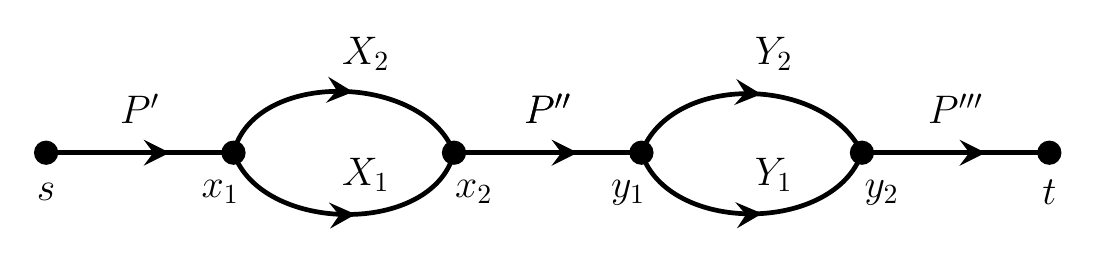
\begin{tikzpicture}[scale=1.40]

\coordinate (p1) at ( 0.0,0);
\coordinate (p2) at ( 1.7,0);
\coordinate (p3) at ( 3.7,0);
\coordinate (p4) at ( 5.4,0);
\coordinate (p5) at ( 7.4,0);
\coordinate (p6) at ( 9.1,0);

\foreach \x in {1,...,6}{\fill (p\x) circle (0.11);}

\node at ($(p1)+( 0.00,-0.36)$) {\Large$s$};
\node at ($(p2)+(-0.12,-0.36)$) {\Large$x_1$};
\node at ($(p3)+(+0.18,-0.36)$) {\Large$x_2$};
\node at ($(p4)+(-0.12,-0.36)$) {\Large$y_1$};
\node at ($(p5)+(+0.18,-0.36)$) {\Large$y_2$};
\node at ($(p6)+( 0.00,-0.36)$) {\Large$t$};

\node at ($(p1)!0.5!(p2)+(0.0, 0.4)$) {\Large$P'$};
\node at ($(p2)!0.5!(p3)+(0.2, 0.9)$) {\Large$X_2$};
\node at ($(p2)!0.5!(p3)+(0.2,-0.2)$) {\Large$X_1$};
\node at ($(p3)!0.5!(p4)+(0.0, 0.4)$) {\Large$P''$};
\node at ($(p3)!0.5!(p4)+(0.0, 0.4)$) {\Large$P''$};
\node at ($(p4)!0.5!(p5)+(0.2, 0.9)$) {\Large$Y_2$};
\node at ($(p4)!0.5!(p5)+(0.2,-0.2)$) {\Large$Y_1$};
\node at ($(p5)!0.5!(p6)+(0.0, 0.4)$) {\Large$P'''$};

\draw[decoration={markings,mark=at position 0.66 with {\arrow[scale=1.5,>=stealth]{>}}},
   postaction={decorate},line width=1.70pt]  (p1)--(p2);
\draw[decoration={markings,mark=at position 0.66 with {\arrow[scale=1.5,>=stealth]{>}}},
   postaction={decorate},line width=1.70pt]  (p3)--(p4);
\draw[decoration={markings,mark=at position 0.66 with {\arrow[scale=1.5,>=stealth]{>}}},
   postaction={decorate},line width=1.70pt]  (p5)--(p6);

\draw[decoration={markings,mark=at position 0.54 with {\arrow[scale=1.5,>=stealth]{>}}},
   postaction={decorate},line width=1.70pt]  (p2) to[out=76,in=111] (p3);
\draw[decoration={markings,mark=at position 0.54 with {\arrow[scale=1.5,>=stealth]{>}}},
   postaction={decorate},line width=1.70pt]  (p2) to[out=-71,in=-104] (p3);

\draw[decoration={markings,mark=at position 0.54 with {\arrow[scale=1.5,>=stealth]{>}}},
   postaction={decorate},line width=1.70pt]  (p4) to[out=69,in=116] (p5);
\draw[decoration={markings,mark=at position 0.54 with {\arrow[scale=1.5,>=stealth]{>}}},
   postaction={decorate},line width=1.70pt]  (p4) to[out=-72,in=-109] (p5);

\end{tikzpicture}
\end{center}
\caption{A 12121-subgraph with the six vertices $s$, $x_1$, $x_2$, $y_1$, $y_2$, and $t$ 
and the seven paths $P'$, $X_1$, $X_2$, $P''$, $Y_1$, $Y_2$, and $P'''$.}
\label{fig:12121}
\medskip
\hrule\hrule
\end{figure}
%%%%%%%%%%%%%%%%%%%%%%%%%%%%%%%%%%%%%%%%%

%%%%%%%%%%%%%%%%%
\begin{lemma}
\label{le:forb.1}
Let $G=(V,A)$ be a directed graph. 
If every path in $\ppp$ possesses a private arc,
then $G$ does not contain any 12121-subgraph.
\end{lemma}
%%%%%%%%%%%%%%%%%
\proof
Suppose for the sake of contradiction that $G$ does contain a 12121-subgraph.
For $i=1,2$ and $j=1,2$, denote by $Q_{ij}$ the path $P'X_iP''Y_jP'''$ in $\ppp$.
As every arc on path $Q_{11}$ is contained in path $Q_{12}$ or in path $Q_{21}$, the path $Q_{11}$
does not possess any private arc.
\qed

\bigskip
The graph depicted in Figure~\ref{fig:bad-example} demonstrates that the 
converse of Lemma~\ref{le:forb.1} does not hold true in general.
This graph contains only four simple directed $s$-$t$-paths: 
$P_1=sv_1t$,
$P_2=sv_2t$,
$P_3=sv_1v_2t$, and
$P_4=sv_2v_1t$.
It is easily verified that the graph does not contain any 12121-subgraph.
Finally, as path $P_1$ shares its first arc $(s,v_1)$ with $P_3$ and as it shares
its second arc $(v_1,t)$ with $P_4$, this path does not possess any private arc.
Summarizing, the absence of the 12121-subgraph does not guarantee the private arc property (P).

%%%%%%%%%%%%%%%%%%%%%%%%%%%%%%%%%%%%%%%%%
\begin{figure}[bth]
\hrule\hrule
\bigskip
\begin{center}
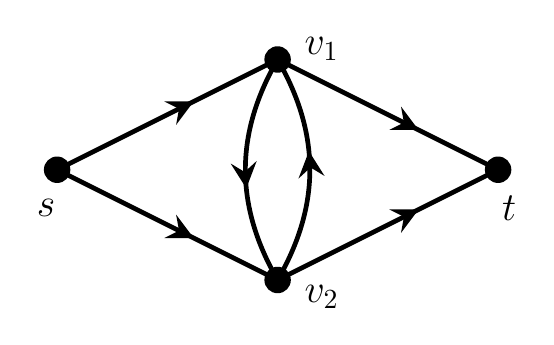
\begin{tikzpicture}[scale=1.40]

\coordinate (p0) at (-2.0, 0.0);
\coordinate (p1) at ( 0.0,+1.0);
\coordinate (p2) at ( 0.0,-1.0);
\coordinate (p3) at (+2.0, 0.0);

\foreach \x in {0,...,3}{\fill (p\x) circle (0.12);}
\node at ($(p0)+(-0.1,-0.35)$) {\Large$s$};
\node at ($(p1)+(+0.4,+0.10)$) {\Large$v_1$};
\node at ($(p2)+(+0.4,-0.15)$) {\Large$v_2$};
\node at ($(p3)+(+0.1,-0.35)$) {\Large$t$};

\foreach \x in {1,2}
  {\draw[decoration={markings,mark=at position 0.62 with {\arrow[scale=1.5,>=stealth]{>}}},
      postaction={decorate},line width=1.70pt] (p0)--(p\x);
   \draw[decoration={markings,mark=at position 0.64 with {\arrow[scale=1.5,>=stealth]{>}}},
      postaction={decorate},line width=1.70pt] (p\x)--(p3);}

\draw[decoration={markings,mark=at position 0.58 with {\arrow[scale=1.5,>=stealth]{>}}},
   postaction={decorate},line width=1.70pt]  (p1) to[out=-120,in=120] (p2);
\draw[decoration={markings,mark=at position 0.58 with {\arrow[scale=1.5,>=stealth]{>}}},
   postaction={decorate},line width=1.70pt]  (p2) to[out=60,in=-60] (p1);

\end{tikzpicture}
\end{center}
\vspace{-4ex}
\caption{A graph without 12121-subgraph that violates the private arc property (P).}
\label{fig:bad-example}
\bigskip
\hrule\hrule
\end{figure}
%%%%%%%%%%%%%%%%%%%%%%%%%%%%%%%%%%%%%%%%%

As the trouble-making graph in Figure~\ref{fig:bad-example} is $\ppp$-covered and 
does contain a directed cycle, its violation of the private arc property could also have 
been concluded from Lemma~\ref{le:no-cycle}.
As it turns out, there are only two types of $\ppp$-covered graphs without 12121-subgraph:
One type does contain a directed cycle, and is not universally linearizable by Lemma~\ref{le:no-cycle}.
The other type is acyclic, and is universally linearizable by Theorem~\ref{th:private} and 
the following Lemma~\ref{le:forb.2}.
%%%%%%%%%%%%%%%%%
\begin{lemma}
\label{le:forb.2}
Let $G=(V,A)$ be an acyclic directed graph.
If $G$ does not contain any 12121-subgraph,
then every path in $\ppp$ possesses a private arc.
\end{lemma}
%%%%%%%%%%%%%%%%%
\proof
Consider some fixed path $P\in\ppp$ that traverses the vertices $v_1,v_2,\ldots,v_p$ in 
that order (where $v_1=s$ and $v_p=t$).
For integers $\alpha$ and $\beta$ with $1\le\alpha<\beta\le p$, we say that the closed interval 
$[\alpha,\beta]$ on the real line is \emph{nice}, if there exists a simple directed path 
$Q[v_{\alpha},v_{\beta}]$ that leads from vertex $v_{\alpha}$ to vertex $v_{\beta}$, that does 
not have any arc in common with path $P$, and whose inner vertices do not belong to path~$P$.
Suppose for the sake of contradiction that there exist two nice intervals $[\alpha,\beta]$ and $[\gamma,\delta]$ 
with $\beta\le\gamma$.
Since graph $G$ is acyclic, the two underlying paths $Q[v_{\alpha},v_{\beta}]$ and $Q[v_{\gamma},v_{\delta}]$ 
are arc-disjoint and do not share any inner vertices.
Then $G$ contains a 12121-subgraph with $x_1=v_{\alpha}$, $x_2=v_{\beta}$, $y_1=v_{\gamma}$, and $y_2=v_{\delta}$;
the seven paths in the 12121-subgraph are the five subpaths that result from cutting path $P$ 
at the vertices $v_{\alpha},v_{\beta},v_{\gamma},v_{\delta}$ together with the two paths 
$Q[v_{\alpha},v_{\beta}]$ and $Q[v_{\gamma},v_{\delta}]$.
This contradiction yields that any two nice intervals $[\alpha,\beta]$ and $[\gamma,\delta]$ 
must intersect \emph{properly} in an interval of length at least~$1$.

Now let $Q\ne P$ be another path in $\ppp$ that shares some common vertex or some common arc with path~$P$. 
As graph $G$ is acyclic, path $Q$ will traverse its common vertices and arcs with $P$ in exactly 
the same order as $P$.
Let $x$ be the largest  index for which the prefix paths $P[s,v_x]$ and $Q[s,v_x]$ coincide, and
let $y$ be the smallest index for which the suffix paths $P[v_y,t]$ and $Q[v_y,t]$ coincide.
Note that the sub-path $Q[v_x,v_y]$ does only share its start-vertex and end-vertex with $P$, 
whereas its inner vertices and its arcs are disjoint from $P$ (as any further overlap or intersection 
between paths $P$ and $Q$ would yield two nice intervals that do not intersect properly).
We associate the nice interval $I(Q):=[x,y]$ with path $Q$.

Finally let ${\cal Q}\subseteq\ppp$ denote the set of all paths $Q\in\ppp$ that share some arc with path $P$
(if there is no such path $Q$, then every arc on $P$ is private and we are done).
By the above discussion, for any two paths $Q_1$ and $Q_2$ in ${\cal Q}$ the two associated nice 
intervals $I(Q_1)$ and $I(Q_2)$ do intersect properly.
Then the one-dimensional version of Helly's theorem \cite{Helly1923} yields that the intersection of all the 
intervals $I(Q)$ with $Q\in{\cal Q}$ is non-empty and forms an interval $[x^*,y^*]$ of length at least~$1$.
As the arc $(v_{x^*},v_{x^*+1})$ lies in every interval $I(Q)$ with $Q\in{\cal Q}$, this arc does 
not belong to any path $Q\in{\cal Q}$ and thus constitutes the desired private arc for path $P$.
\qed

\bigskip
In the rest of this section, we use Lemmas~\ref{le:forb.1} and \ref{le:forb.2} to get a better 
understanding of acyclic directed graphs $G=(V,A)$ that are universally linearizable.
In such a graph every vertex $v\in V-\{s,t\}$ has at least one in-going arc (as vertex $s$ is the 
unique source) and at least one out-going arc (as vertex $t$ is the unique sink).
We classify the vertices in $V-\{s,t\}$ into four subsets $V_{11}$, $V_{12}$, $V_{21}$, and $V_{22}$:
\begin{itemize}
\item The vertices in $V_{11}$ have in-degree $1$ and out-degree $1$.
\item The vertices in $V_{12}$ have in-degree $1$ and out-degree at least $2$.
\item The vertices in $V_{21}$ have in-degree at least $2$ and out-degree $1$.
\item The vertices in $V_{22}$ have both in-degree and out-degree at least $2$.
\end{itemize}
%%%%%%%%%%%%%%%%%
\begin{lemma}
\label{le:D1D2}
An acyclic graph $G=(V,A)$ with unique source and unique sink is universally linearizable, 
if and only if it satisfies the following two conditions:
\begin{quote}
\begin{itemize}
\item[(D1)] The vertex set $V_{22}$ is empty.
\item[(D2)] No directed path connects a vertex in $V_{21}$ to a vertex in $V_{12}$.
\end{itemize}
\end{quote}
\end{lemma}
%%%%%%%%%%%%%%%%%
\proof
First suppose that the acyclic graph $G$ is not universally linearizable, and hence 
by Theorem~\ref{th:private} and Lemma~\ref{le:forb.2} does contain a 12121-subgraph.
If the vertices $x_2$ and $y_1$ in the 12121-subgraph coincide, there is a vertex in $V_{22}$
and (D1) is violated.
If the vertices $x_2$ and $y_1$ in the subgraph are distinct, they and their connecting
path $P''$ violate condition~(D2).

Next suppose that $G$ is universally linearizable.
If some vertex $v$ has two in-going arcs $(u_1,v)$ and $(u_2,v)$, there are two 
paths $P_1$ and $P_2$ that connect $s$ to $u_1$ and $u_2$.
If $v$ also has two out-going arcs $(v,w_1)$ and $(v,w_2)$, there are two further
paths $Q_1$ and $Q_2$ that connect $w_1$ and $w_2$ to $t$.
Since $G$ is acyclic, we can construct a 12121-subgraph in $G$ that results by pasting together 
appropriate pieces of $P_1$, $P_2$, $Q_1$ and $Q_2$.
Lemma~\ref{le:forb.1} shows that such a vertex $v$ does not exist, and hence yields (D1).
If there is a simple path $P_0$ that connects some vertex $x\in V_{21}$ to some vertex $y\in V_{12}$,
then there are two paths $P_1$ and $P_2$ that connect $s$ to $x$ and that use two distinct 
arcs going into $x$; furthermore there are two paths $Q_1$ and $Q_2$ that connect $y$ to $t$ and 
that use two distinct arcs out of $y$.
Then we can construct a 12121-subgraph by pasting together appropriate pieces of 
$P_0$, $P_1$, $P_2$, $Q_1$ and $Q_2$.
Hence such vertices $x$ and $y$ do not exist, and (D2) holds.
\qed

\bigskip
Lemma~\ref{le:D1D2} leads to yet another, extremely simple combinatorial characterization of 
universally linearizable acyclic graphs $G=(V,A)$.
Let us consider a path $P\in\ppp$ on the vertices $v_1,v_2,\ldots,v_p$ in that order 
(where $v_1=s$ and $v_p=t$).
By condition (D2), on path $P$ every vertex in $V_{12}$ precedes every vertex in $V_{21}$.
Hence by (D1) and (D2), there exists an arc $(v_k,v_{k+1})$ with $1\le k\le p-1$, 
whose removal divides path $P$ 
into a prefix path on vertices $v_1,    \ldots,v_k\in\{s\}\cup V_{11}\cup V_{12}$ and
into a suffix path on vertices $v_{k+1},\ldots,v_p\in\{t\}\cup V_{11}\cup V_{21}$.
The first arc with that property on $P$ is denoted $a^*(P)$.
It is easily seen that $a^*(P)$ is a private arc for path $P$.
Now let us remove the private arc $a^*(P)$ from every path $P\in\ppp$.
The remaining graph consists of a component with vertices from $\{s\}\cup V_{11}\cup V_{12}$ 
that are reachable from the source $s$, and of another component with vertices from 
$\{t\}\cup V_{11}\cup V_{21}$ from which the sink~$t$ can be reached.
This yields that an acyclic universally linearizable graph $G$ is structured 
into three parts as follows.
\begin{itemize}
\item There is an out-tree $T^+$ whose root is $s$, and whose inner vertices 
are the vertices in $V_{12}$ together with some subset of the vertices in $V_{11}$.
\item There is an  in-tree $T^-$ whose root is $t$, and whose inner vertices 
are the vertices in $V_{21}$ together with the remaining vertices in $V_{11}$.
\item Finally there are the arcs $a^*(P)$ with $P\in\ppp$. Each of these arcs connects
a vertex in the out-tree $T^+$ to a vertex in the in-tree $T^-$.
\end{itemize}
With this knowledge, it is straightforward to see that the acyclic graph shown 
in Figure~\ref{fig:example2} is indeed universally linearizable:
The out-tree $T^+$ is induced by the three vertices $s,v_1,v_2$, and
the  in-tree $T^-$ is induced by the three vertices $v_3,v_4,t$.
The remaining four arcs connect $T^+$ to $T^-$, and hence form the private arcs of the paths in $\ppp$.

\bigskip
The following theorem summarizes the results of this section on acyclic graphs and 
combines them with Theorem~\ref{th:private}.
The degree condition (D) compresses the two conditions (D1) and (D2) from Lemma~\ref{le:D1D2} into 
a single condition (D); note in particular that (D) implies (D1) via paths of length zero.
The tree condition (T) summarizes the discussion on in-trees and out-trees in the preceding paragraphs.
%%%%%%%%%%%%%%%%%
\begin{theorem}
\label{th:acyclic}
For a directed acyclic graph $G=(V,A)$ with unique source and unique sink, 
the following five statements are pairwise equivalent:
\begin{quote}
\begin{itemize}
\itemsep=0.9ex
\item[(U)] Graph $G$ is universally linearizable.
\item[(P)] Every path in $\ppp$ possesses a private arc.
\item[(F)] Graph $G$ does not contain any 12121-subgraph.
\item[(D)] There is no directed path that leads from a vertex with in-degree 
at least~$2$ to a vertex with out-degree at least $2$.
\item[(T)] Graph $G$ consists of an out-tree rooted at $s$, an in-tree rooted at $t$,
and of several arcs that connect the out-tree to the in-tree.
\end{itemize}
\end{quote}
\end{theorem}
%%%%%%%%%%%%%%%%%


%%%%%%%%%%%%%%%%%%%%%%%%%%%%%%%%%%%%%%%%%%%%%%%%%%%%%%%%%%%%%%%%%%%%%%%%%
%%%%%%%%%%%%%%%%%%%%%%%%%%%%%%%%%%%%%%%%%%%%%%%%%%%%%%%%%%%%%%%%%%%%%%%%%
\medskip
\section{The recognition of universally linearizable graphs}
\label{sec:algo}
%%%%%%%%%%%%%%%%%%%%%%%%%%%%%%%%%%%%%%%%%%%%%%%%%%%%%%%%%%%%%%%%%%%%%%%%%
In this section we present fast, polynomial time recognition algorithms for
universally linearizable graphs.
Since the algorithmic side of $\ppp$-covered graphs is not well-understood 
(see Section~\ref{sec:conclusion} for a discussion of this issue), we will not a priori 
assume that the graphs considered in this section are $\ppp$-covered.

%%%%%%%%%%%%%%%%%
\begin{lemma}
\label{le:algo-acyclic}
For a given acyclic directed graph $G=(V,A)$ with unique source and unique sink, 
it can be decided in linear time $O(|V|+|A|)$ whether $G$ is universally linearizable.
\end{lemma}
%%%%%%%%%%%%%%%%%
\proof
We check whether the graph satisfies conditions (D1) and (D2) in Lemma~\ref{le:D1D2}.
In an $O(|V|+|A|)$ preprocessing phase, we compute for every vertex in $V$ its in-degree and out-degree.
Then condition (D1) can be deduced directly from the in-degrees and out-degrees.
For condition (D2), we have to determine the vertices that can be reached from the set $V_{21}$.
This is a reachability problem that can easily be solved in $O(|V|+|A|)$ time by routine methods; 
see for instance \cite{CLRS}.
\qed

\bigskip
The proof of the following theorem uses a well-known algorithm by Read \& Tarjan \cite{ReTa1975} 
for listing the simple directed $s$-$t$-paths in a directed graph $G=(V,A)$.
The algorithm takes $O(|V|+|A|+k|A|)$ time, where $k$ is the number of paths to be listed.
We will apply this algorithm to find out whether the graph does contain $k\ge\ell$ paths for
a given bound $\ell$, within $O(|V|+|A|+\ell|A|)$ time:
Once the running time of the algorithm exceeds a certain bound (that depends on the implementation,
but is easy to compute), we simply terminate the algorithm and conclude $k\ge\ell$.
%%%%%%%%%%%%%%%%%
\begin{theorem}
\label{th:algo}
For a given (not necessarily $\ppp$-covered) directed graph $G=(V,A)$ with unique source and 
unique sink, it can be decided in polynomial time $O(|V|\cdot|A|^2)$ 
whether $G$ is universally linearizable.
\end{theorem}
%%%%%%%%%%%%%%%%%
\proof
By Theorem~\ref{th:private}, a graph $G$ is universally linearizable if and only if 
every path in $\ppp$ contains some private arc.
If the algorithm of Read \& Tarjan \cite{ReTa1975} manages to find $\ell:=|A|+1$ different 
$s$-$t$-paths in $O(|V|\cdot|A|^2)$ time, we immediately output NO and stop: $|A|+1$ different 
paths need $|A|+1$ different private arcs, whereas the graph only has $|A|$ different arcs.
In the remaining cases, the algorithm finds at most $|A|$ simple paths that each consist of at most $|A|$ arcs.
It is straightforward to check in $O(|A|^2)$ time whether each of these paths possesses 
a private arc.
\qed


%%%%%%%%%%%%%%%%%%%%%%%%%%%%%%%%%%%%%%%%%%%%%%%%%%%%%%%%%%%%%%%%%%%%%%%%%
%%%%%%%%%%%%%%%%%%%%%%%%%%%%%%%%%%%%%%%%%%%%%%%%%%%%%%%%%%%%%%%%%%%%%%%%%
\medskip
\section{The recognition of linearizable QSPP instances}
\label{sec:hardness}
%%%%%%%%%%%%%%%%%%%%%%%%%%%%%%%%%%%%%%%%%%%%%%%%%%%%%%%%%%%%%%%%%%%%%%%%%
While the preceding sections investigated the structure of graphs for the QSPP, 
the current section will analyze full QSPP instances (that do specify both, the 
graph and the arc interaction costs).
Hu \& Sotirov \cite{HuSo2018b} have shown that the decision problems VALID-LI\-NEARI\-ZA\-TION
and LI\-NEA\-RIZABLE-QSPP in Figure~\ref{fig:problems} both are polynomially solvable, 
if the underlying directed graph $G$ is acyclic.
The following (purely combinatorial) proposition can be extracted and deduced from the algorithmic
arguments in \cite{HuSo2018b}, by combining them with the techniques of our Section~\ref{sec:forbidden}.
For subsets $S,T\subseteq A$ of the arc set we denote $q(S,T)=\sum_{s\in S}\sum_{t\in T}q(s,t)$.

%%%%%%%%%%%%%%%%%%%%%%%%%%%%%%%%%%%%%%%%%%%%%%%%%%
\begin{figure}[tb]
\begin{center}
%%%%%%%%%%%%%%%%%
\boxxx{Problem: VALID-LINEARIZATION
\\[2.0ex]
Instance: A $\ppp$-covered directed graph $G=(V,A)$ with $s,t\in V$;
arc interaction costs $q:A\times A\to\RRR$; weights $w:A\to\RRR$.
\\[2.0ex]
Question: Do the arc weights $w$ form a valid linearization of the given
QSPP instance $G$ and $q$?}
%%%%%%%%%%%%%%%%%

\bigskip
\bigskip
%%%%%%%%%%%%%%%%%
\boxxx{Problem: LINEARIZABLE-QSPP
\\[2.0ex]
Instance: A $\ppp$-covered directed graph $G=(V,A)$ with $s,t\in V$;
arc interaction costs $q:A\times A\to\RRR$.
\\[2.0ex]
Question: Does there exist a linearization $w:A\to\RRR$ for this QSPP instance?}
%%%%%%%%%%%%%%%%%
\end{center}
\caption{The decision problems discussed in Section~\protect{\ref{sec:hardness}}.}
\label{fig:problems}
\medskip
\hrule\hrule
\end{figure}
%%%%%%%%%%%%%%%%%%%%%%%%%%%%%%%%%%%%%%%%%%%%%%%%%%

%%%%%%%%%%%%%%%%%
\begin{proposition}
\label{pr:HS}
For an acyclic directed graph $G=(V,A)$ with $s,t\in V$ and for arc interaction
costs $q:A\times A\to\RRR$, the following two statements are equivalent.
\begin{quote}
\begin{itemize}
\item[(L1)] The QSPP instance $G$ and $q$ is linearizable.
\item[(L2)] In every 12121-subgraph of $G$, the subpaths $X_1,X_2,Y_1,Y_2$ satisfy the equation
$q(X_1,Y_1)+q(X_2,Y_2) = q(X_1,Y_2)+q(X_2,Y_1)$.
\end{itemize}
\end{quote}
\end{proposition}
%%%%%%%%%%%%%%%%%

In this section we will show that the problems VALID-LINEARIZATION and LI\-NEA\-RIZ\-ABLE-QSPP
both are coNP-complete in arbitrary (not necessarily acyclic) directed graphs.
Note that the combinatorial characterization in Proposition~\ref{pr:HS} yields a coNP-certificate 
for the (polynomially solvable) special case of problem LINEARIZABLE-QSPP on acyclic graphs:
Any NO-instance contains a 12121-subgraph whose subpaths $X_1,X_2,Y_1,Y_2$ violate the equation in (L2).
Unfortunately this coNP-certificate does not generalize to graphs with cycles, as the 
following example demonstrates.
Consider the graph on six vertices $s,t,x_1,x_2,x_3,y$ in Figure~\ref{fig:trefoil}, 
and define arc interaction costs as follows:
The interaction cost of the two arcs $(x_1,y)$ and $(y,x_2)$ is $1$; 
the interaction cost of the two arcs $(x_2,y)$ and $(y,x_3)$ is $1$; and
the interaction cost of the two arcs $(x_3,y)$ and $(y,x_1)$ is $1$;
all other arc interaction costs are~$0$.
As the graph does not contain any 12121-subgraph, the QSPP instance trivially satisfies 
condition (L2) in Proposition~\ref{pr:HS}.
However, this instance is not linearizable and hence violates condition (L1):
The three paths 
$P_1=sx_1yx_2t$, 
$P_2=sx_2yx_3t$,
$P_3=sx_3yx_1t$
together traverse each of the twelve arcs exactly once, and the three paths
$Q_1=sx_1yx_3t$,
$Q_2=sx_2yx_1t$,
$Q_3=sx_3yx_2t$
together also traverse each of the twelve arcs exactly once.
Therefore any linear weight function $w:A\to\RRR$ will satisfy $\sum_{i=1}^3\spp(P_i,w)=\sum_{i=1}^3\spp(Q_i,w)$,
which badly collides with $\sum_{i=1}^3\qspp(P_i,q)=6$ and $\sum_{i=1}^3\qspp(Q_i,q)=0$.
The following lemma constructs a coNP-certificate for LINEARIZABLE-QSPP that is based on a 
different approach.

%%%%%%%%%%%%%%%%%%%%%%%%%%%%%%%%%%%%%%%%%
\begin{figure}[bth]
\hrule\hrule
\bigskip
\medskip
\begin{center}
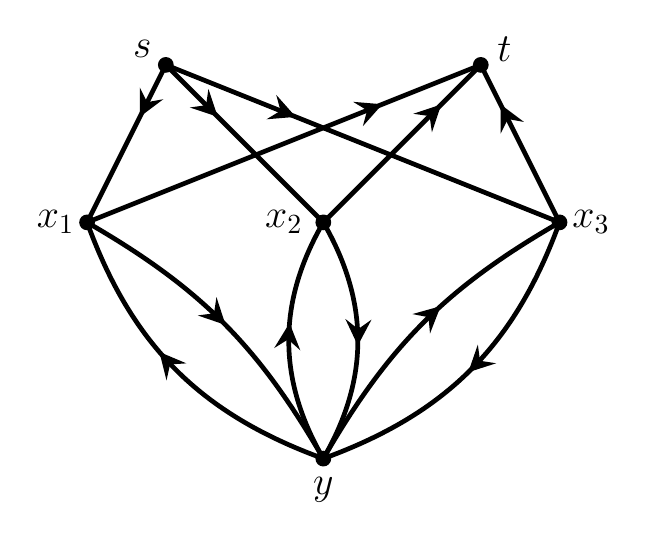
\begin{tikzpicture}[scale=1.00]

\coordinate (p1) at (-2.0, 4.0);
\coordinate (p2) at (+2.0, 4.0);
\coordinate (p3) at ( 0.0,-1.0);
\coordinate (q1) at (-3.0, 2.0);
\coordinate (q2) at ( 0.0, 2.0);
\coordinate (q3) at (+3.0, 2.0);

\foreach \x in {1,...,3}{\fill (p\x) circle (0.10);}
\foreach \x in {1,...,3}{\fill (q\x) circle (0.10);}

\node at ($(p1)+(-0.3, 0.20)$) {\Large$s$};
\node at ($(p2)+(+0.3, 0.20)$) {\Large$t$};
\node at ($(p3)+( 0.0,-0.40)$) {\Large$y$};
\node at ($(q1)+(-0.4, 0.00)$) {\Large$x_1$};
\node at ($(q2)+(-0.5, 0.00)$) {\Large$x_2$};
\node at ($(q3)+(+0.4, 0.00)$) {\Large$x_3$};

\foreach \x in {1,...,3}
  {\draw[decoration={markings,mark=at position 0.33 with {\arrow[scale=1.5,>=stealth]{>}}},
      postaction={decorate},line width=1.70pt] (p1)--(q\x);
   \draw[decoration={markings,mark=at position 0.75 with {\arrow[scale=1.5,>=stealth]{>}}},
      postaction={decorate},line width=1.70pt] (q\x)--(p2);}

\draw[decoration={markings,mark=at position 0.57 with {\arrow[scale=1.5,>=stealth]{>}}},
   postaction={decorate},line width=1.70pt]  (p3) to[out=160,in=-70] (q1);
\draw[decoration={markings,mark=at position 0.51 with {\arrow[scale=1.5,>=stealth]{>}}},
   postaction={decorate},line width=1.70pt]  (q1) to[out=-30,in=120] (p3);

\draw[decoration={markings,mark=at position 0.57 with {\arrow[scale=1.5,>=stealth]{>}}},
   postaction={decorate},line width=1.70pt]  (p3) to[out=120,in=-120] (q2);
\draw[decoration={markings,mark=at position 0.52 with {\arrow[scale=1.5,>=stealth]{>}}},
   postaction={decorate},line width=1.70pt]  (q2) to[out=-60,in=60] (p3);

\draw[decoration={markings,mark=at position 0.57 with {\arrow[scale=1.5,>=stealth]{>}}},
   postaction={decorate},line width=1.70pt]  (p3) to[out=60,in=-150] (q3);
\draw[decoration={markings,mark=at position 0.51 with {\arrow[scale=1.5,>=stealth]{>}}},
   postaction={decorate},line width=1.70pt]  (q3) to[out=-110,in=20] (p3);

\end{tikzpicture}
\end{center}
\vspace{-4ex}
\caption{Proposition~\protect{\ref{pr:HS}} does not generalize to graphs with cycles.}
\label{fig:trefoil}
\bigskip
\hrule\hrule
\end{figure}
%%%%%%%%%%%%%%%%%%%%%%%%%%%%%%%%%%%%%%%%%


%%%%%%%%%%%%%%%%%
\begin{lemma}
\label{le:coNP}
The problems VALID-LINEARIZATION and LINEARIZABLE-QSPP are contained in the complexity class coNP.
\end{lemma}
%%%%%%%%%%%%%%%%%
\proof
Every NO-instance of VALID-LINEARIZATION contains some path $P$ that violates the condition
$\qspp(P,q)=\spp(P,w)$ in \eqref{eq:linearizable}.
This path $P$ is the coNP-certificate: The path can be described with polynomially many bits,
and its violation of \eqref{eq:linearizable} is easily verified in polynomial time.
Hence VALID-LINEARIZATION is contained in coNP.

Next let us consider a NO-instance of LINEARIZABLE-QSPP.
This means that the following system of linear equations and inequalities with real 
variables $w_a$ for the arcs $a\in A$ is infeasible:
%%%%%%%%%%%%%%%%
\begin{align}
\sum_{a\in P} w_a~=~\qspp(P,q) &\qquad\text{for every path $P\in\ppp$} \label{eq:lp.1} \\[-1.2ex]
              w_a~\ge~0        &\qquad\text{for every arc $a\in A$}    \label{eq:lp.2} \\[-2.5ex]
\hphantom{\sum_{P\in\ppp} \qspp(P,q)\cdot x_P~<~0} &&                  \nonumber
\end{align}
%%%%%%%%%%%%%%%%
By Farkas' lemma \cite{Farkas1902}, the infeasibility of the system \eqref{eq:lp.1}--\eqref{eq:lp.2}
is equivalent to the feasibility of the following dual system with real variables $x_P$ for the
paths $P\in\ppp$:
%%%%%%%%%%%%%%%%
\begin{align}
\sum_{P\in\ppp} \qspp(P,q)\cdot x_P ~<~0 &                                    \label{eq:dlp.1} \\[-0.2ex]
\sum_{P:\,a\in P} x_P             ~\ge~0 &\qquad\text{for every arc $a\in A$} \label{eq:dlp.2} 
\end{align}
%%%%%%%%%%%%%%%%
Now fix some feasible solution $x^*$ for \eqref{eq:dlp.1}--\eqref{eq:dlp.2},
let $\pppx$ denote the set of all paths $P\in\ppp$ with $x^*_P\ge0$, and 
let $\pppy$ denote the set of all paths $P\in\ppp$ with $x^*_P<0$.
We introduce the following additional constraints:
%%%%%%%%%%%%%%%%
\begin{align}
\sum_{P\in\pppx}x_P - \sum_{P\in\pppy}x_P  ~\le~1  &                 \label{eq:dlp.3} \\[-0.5ex]
                x_P  ~\ge~0 &\qquad\text{for every path $P\in\pppx$} \label{eq:dlp.4} \\[0.5ex]
                x_P  ~\le~0 &\qquad\text{for every path $P\in\pppy$} \label{eq:dlp.5} \\[-2.5ex] 
\hphantom{\sum_{P\in\ppp} \qspp(P,q)\cdot x_P~<~0} &&                \nonumber
\end{align}
%%%%%%%%%%%%%%%%
As the constraints \eqref{eq:dlp.3}--\eqref{eq:dlp.5} enforce $|x_P|\le1$ for every path $P$, 
the underlying feasible region is bounded.
Furthermore it is easy to see that the feasibility of the system \eqref{eq:dlp.1}--\eqref{eq:dlp.2} 
implies the feasibility of the system \eqref{eq:dlp.1}--\eqref{eq:dlp.5}.
In particular, the system \eqref{eq:dlp.1}--\eqref{eq:dlp.5} possesses a feasible solution $x^{**}$ 
that satisfies the strict inequality \eqref{eq:dlp.1}, and 
that furthermore is a corner vertex of the polytope defined by \eqref{eq:dlp.2}--\eqref{eq:dlp.5}.
As we are working in $|\ppp|$-dimensional space, the corner vertex $x^{**}$ satisfies $|\ppp|$ of 
the constraints \eqref{eq:dlp.2}--\eqref{eq:dlp.5} with equality; this implies that at most $|A|+1$ 
of the coordinates in $x^{**}$ are non-zero.

Now our coNP-certificate for LINEARIZABLE-QSPP simply lists all the paths $P\in\ppp$ with $x^{**}_P\ne0$.
As the certificate consists of at most $|A|+1$ paths that each contain at most $|A|$ arcs, the
size of the certificate is polynomially bounded in the instance size.
The certificate is verified in polynomial time as follows:
We consider the restriction of the system \eqref{eq:lp.1}--\eqref{eq:lp.2} to the paths $P$ 
in the certificate.
As this restricted system has a polynomial number of variables and a polynomial number of constraints,
it can be solved (and found to be infeasible) in polynomial time by linear programming.
Hence LINEARIZABLE-QSPP is indeed contained in coNP.
\qed

\bigskip
The coNP-hardness proofs will be done by reductions from the following problem TWO-VERTEX-DISJOINT-PATHS.
%%%%%%%%%%%%%%%%%
\begin{quote}
Problem: TWO-VERTEX-DISJOINT-PATHS
\\[1.0ex]
Instance: A directed graph $H=(V_H,A_H)$ with two sources $s_1,s_2\in V$ and two sinks $t_1,t_2\in V$.
\\[1.0ex]
Question: Do there exist two vertex-disjoint simple directed paths $P_1$ and $P_2$ in $H$,
so that path $P_1$ goes from $s_1$ to $t_1$ and path $P_2$ goes from $s_2$ to $t_2$?
\end{quote}
%%%%%%%%%%%%%%%%%
The NP-hardness of TWO-VERTEX-DISJOINT-PATHS has been established by Fortune, Hopcroft \& Wyllie \cite{FoHoWy1980}.
By scrutinizing the reduction in \cite{FoHoWy1980}, we actually get the slightly stronger statement
in the following proposition.
%%%%%%%%%%%%%%%%%
\begin{proposition}
\label{pr:FHW}
\cite{FoHoWy1980}
The problem TWO-VERTEX-DIS\-JOINT-PATHS is NP-hard, even on directed graphs $H=(V_H,A_H)$
\begin{itemize}
\item where every arc in $A_H$ is contained in some simple directed path from $s_1$ to~$t_1$ 
or in some simple directed path from $s_2$ to~$t_2$, and
\item where there is at least one simple directed path from $s_1$ to~$t_1$ 
and at least one simple directed path from $s_2$ to~$t_2$.
\end{itemize}
\end{proposition}
%%%%%%%%%%%%%%%%%

We consider an instance of TWO-VERTEX-DISJOINT-PATHS as in Proposition~\ref{pr:FHW},
and create from it a corresponding instance of QSPP.
The underlying directed graph $G=(V,A)$ is defined as follows.
\begin{itemize}
\item The vertex set $V$ consists of all vertices in $V_H$, of a primed copy $v'$ of every
vertex $v\in V_H$, and of three additional vertices $s$, $t$, and $z$.
\item The arc set $A$ contains all arcs in $A_H$ together with a primed copy $(u',v')$
of every arc $(u,v)\in A_H$.
Furthermore, the arc set $A$ contains
the two arcs $a_1$ and $a'_1$ from $s$ to $s_1$ and $s'_1$,
the two arcs $b_1$ and $b'_1$ from $t_1$ and $t'_1$ to $z$,
the two arcs $a_2$ and $a'_2$ from $z$ to $s_2$ and $s'_2$, and finally
the two arcs $b_2$ and $b'_2$ from $t_2$ and $t'_2$ to $t$.
\end{itemize}
All the arc interaction costs are set to $0$, with only two exceptions:
The interaction cost of the two arcs $b_1=(t_1,z)$ and $a_2=(z,s_2)$ equals $1$, and
the interaction cost of the two arcs $b'_1=(t'_1,z)$ and $a'_2=(z,s'_2)$ equals $1$.
This completes the description of the QSPP instance.

Note that the constructed graph $G=(V,A)$ indeed is $\ppp$-covered:
If an arc $a\in A_H$ lies on a simple directed path $P_a$ from $s_1$ to~$t_1$ in $H$,
graph $G$ contains the simple path that starts in $s$, traverses path $P_a$ in $H$, moves on to $z$,
traverses some simple path from $s'_2$ to $t'_2$ in the primed subgraph, and ends in $t$.
The cases where arc $a\in A_H$ lies on a simple directed path from $s_2$ to~$t_2$ in $H$ 
and the cases where an arc lies in the primed subgraph are settled by symmetric arguments.
%%%%%%%%%%%%%%%%%
\begin{lemma}
\label{le:hard.1}
If the instance of TWO-VERTEX-DISJOINT-PATHS has answer YES,
then the constructed instance of QSPP is not linearizable.
\end{lemma}
%%%%%%%%%%%%%%%%%
\proof
Suppose for the sake of contradiction that there would exist a linearization~$w$.
Let $P_1$ and $P_2$ be the two vertex disjoint paths in graph $H$, and let $P'_1$ and $P'_2$
be the corresponding primed copies of these two paths through the primed vertices.
By considering 
the simple path $s-P_1-z-P_2-t$,  
the simple path $s-P_1-z-P'_2-t$,  
the simple path $s-P'_1-z-P_2-t$, and 
the simple path $s-P'_1-z-P'_2-t$, 
we get the following system of equations for the weights $w$ in the linearization:
%%%%%%%%%%%%%%%%
\begin{eqnarray}
w(a_1) +w(P_1 )+w(b_1) +w(a_2) +w(P_2 )+w(b_2)  &=& 2 \label{eq:x11} \\[0.5ex]
w(a_1) +w(P_1 )+w(b_1) +w(a'_2)+w(P'_2)+w(b'_2) &=& 0 \label{eq:x12} \\[0.5ex]
w(a'_1)+w(P'_1)+w(b'_1)+w(a_2) +w(P_2 )+w(b_2)  &=& 0 \label{eq:x21} \\[0.5ex]
w(a'_1)+w(P'_1)+w(b'_1)+w(a'_2)+w(P'_2)+w(b'_2) &=& 2 \label{eq:x22} 
\end{eqnarray}
%%%%%%%%%%%%%%%%
If we multiply \eqref{eq:x11}, \eqref{eq:x12}, \eqref{eq:x21}, \eqref{eq:x22}
respectively by the values $+1$, $-1$, $-1$, $+1$ and add up the resulting equations,
we arrive at the desired contradiction.
\qed

%%%%%%%%%%%%%%%%%
\begin{lemma}
\label{le:hard.2} 
If the instance of TWO-VERTEX-DISJOINT-PATHS has answer NO,
then the constructed instance of QSPP can be linearized by setting weight $w(a)=0$ for every arc $a\in A$.
\end{lemma}
%%%%%%%%%%%%%%%%% 
\proof
Suppose for the sake of contradiction that $w$ is not a valid linearization and hence 
violates the statement in~\eqref{eq:linearizable}.
As in the linearization all paths $P\in\ppp$ satisfy $\spp(P,w)=0$, the violation must
be caused by some path with $\qspp(P,q)>0$.
Such a path $P$ either contains (i) the two arcs $b_1=(t_1,z)$ and $a_2=(z,s_2)$ or 
(ii) the two arcs $b'_1=(t'_1,z)$ and $a'_2=(z,s'_2)$.
In case~(i) path $P$ starts in $s$, traverses a simple path $P_1$ from $s_1$ to $t_1$ 
in the subgraph $H$, then jumps to vertex $z$, then traverses a simple path $P_2$ from 
$s_2$ to $t_2$ in the subgraph $H$, and ends in $t$.
Since the two paths $P_1$ and $P_2$ are vertex-disjoint, they constitute a solution for 
the TWO-VERTEX-DISJOINT-PATHS instance; hence we get the desired contradiction.
In case~(ii) we derive an analogous contradiction in the primed copy of graph $H$.
\qed

%%%%%%%%%%%%%%%%%
\begin{theorem}
\label{th:hard}
The problems VALID-LINEARIZATION and LINEARIZABLE-QSPP are coNP-complete.
\end{theorem}
%%%%%%%%%%%%%%%%%
\proof
By Lemma~\ref{le:coNP} both problems are contained in coNP.
For the coNP-hardness of LINEARIZABLE-QSPP, our reduction uses the constructed instance of QSPP.
For the coNP-hardness of VALID-LINEARIZATION, our reduction uses the constructed instance of QSPP
together with the arc weights $w(a)=0$ for all arcs $a\in A$.
Lemmas~\ref{le:hard.1} and~\ref{le:hard.2} yield the correctness of both reductions.
\qed


%%%%%%%%%%%%%%%%%%%%%%%%%%%%%%%%%%%%%%%%%%%%%%%%%%%%%%%%%%%%%%%%%%%%%%%%%
%%%%%%%%%%%%%%%%%%%%%%%%%%%%%%%%%%%%%%%%%%%%%%%%%%%%%%%%%%%%%%%%%%%%%%%%%
\medskip
\section{Conclusion}
\label{sec:conclusion}
%%%%%%%%%%%%%%%%%%%%%%%%%%%%%%%%%%%%%%%%%%%%%%%%%%%%%%%%%%%%%%%%%%%%%%%%%
We have provided a number of characterizations of universally linearizable graphs for the QSPP.
In particular, we have shown that such graphs can be recognized in polynomial time,
and that a $\ppp$-covered universally linearizable graph must be acyclic. 
There seems to be a close connection between the QSPP on acyclic graphs and 12121-subgraphs,
as illustrated by Theorem~\ref{th:acyclic} and Proposition~\ref{pr:HS}.
As a rule of thumb, problems around the linearization of the QSPP (as for instance 
the problems LINEARIZABLE-QSPP and VALID-LINEARIZATION in Section~\ref{sec:hardness}) 
are well-behaved and tractable in acyclic graphs, whereas they appear to be shambolic 
and intractable in the general case.

We have sometimes assumed that the considered graphs are $\ppp$-covered.
From the combinatorial point of view, this assumption can be made without the slightest loss 
of generality: If an arc is not traversed by any path in $\ppp$, this arc is irrelevant for 
the objective value of the QSPP and hence also irrelevant for the linearizability of the QSPP.
From the algorithmic point of view, however, this assumption of $\ppp$-coveredness can not be 
made without loss of generality.
The property of being $\ppp$-covered (which is delicate and far from trivial) is encapsulated
in the following algorithmic problem:
\emph{``Given a directed graph $G=(V,A)$ and two vertices $s,t\in V$, is this graph $\ppp$-covered?''}
The arguments in Fortune, Hopcroft \& Wyllie \cite{FoHoWy1980} imply that this algorithmic
problem is NP-complete; we remark that this NP-completeness result is not stated explicitly in
\cite{FoHoWy1980}, but can be extracted and deduced from the arguments.
We stress that our hardness results in Section~\ref{sec:hardness} are not corollaries to the 
intractability of recognizing $\ppp$-covered graphs: LINEARIZABLE-QSPP and VALID-LINEARIZATION 
are intractable even in $\ppp$-covered graphs, and they remain intractable even if for every 
arc in $A$ a corresponding covering path is specified as part of the input.

An open problem is to formulate an appropriate weakened version of Proposition~\ref{pr:HS} 
that also applies to cyclic graphs.
Though the graph in Figure~\ref{fig:trefoil} and its subdivisions demonstrate that the 
statement does not apply to all cyclic graphs, we feel that it should be true for most graphs; 
perhaps it is possible to get a clean and simple characterization of the graphs for which the
statement is false.

\medskip
\paragraph{Acknowledgements.}
This research has been supported 
by the Austrian Science Fund (FWF): W1230, Doctoral Program ``Discrete Mathematics'',
and by the DFG RTG 2236 ``UnRAVeL''.


%%%%%%%%%%%%%%%%%%%%%%%%%%%%%%%%%%%%%%%%%%%%%%%%%%%%%%%%%%%%%%%%%%%%%%%%%
%%%%%%%%%%%%%%%%%%%%%%%%%%%%%%%%%%%%%%%%%%%%%%%%%%%%%%%%%%%%%%%%%%%%%%%%%
\medskip
\begin{thebibliography}{18}

\bibitem{Bo1990}
{\sc I. Bookhold} (1990).
A contribution to quadratic assignment problems.
\emph{Optimization 21}, 933--943.

\bibitem{CeDeWo2016}
{\sc E. \c{C}ela, V.G. Deineko, and G.J. Woeginger} (2016).
Linearizable special cases of the {QAP}.
\emph{Journal of Combinatorial Optimization 31}, 1269--1279.

\bibitem{CLRS}
{\sc T.H. Cormen, C.E. Leiserson, R.L. Rivest, and C. Stein} (2001).
\emph{Introduction to Algorithms}.
MIT Press.

\bibitem{CuPu2016}
{\sc A. {\'C}usti{\'c} and A.P. Punnen} (2018).
A characterization of linearizable instances of the quadratic minimum spanning tree problem.
\emph{Journal of Combinatorial Optimization 35}, 436--453.

\bibitem{deMeSo2020}
{\sc F. de Meijer and R. Sotirov} (2020).
The quadratic cycle cover problem: special cases and efficient bounds.
\emph{Journal of Combinatorial Optimization 39}, 1096--1128.

\bibitem{Erdogan2006}
{\sc G. Erdo\u{g}an} (2006).
Quadratic assignment problem: linearizations and polynomial time solvable cases.
PhD Thesis, Department of Industrial Engineering, Bilkent University.

\bibitem{ErTa2007}
{\sc G. Erdo\u{g}an and B.C. Tansel} (2007).
A branch-and-cut algorithm for quadratic assignment problems based on linearizations.
\emph{Computers and Operations Research 34}, 1085--1106.

\bibitem{ErTa2011}
{\sc G. Erdo\u{g}an and B.C. Tansel} (2011).
Two classes of quadratic assignment problems that are solvable as linear assignment problems.
\emph{Discrete Optimization 8}, 446--451.

\bibitem{Farkas1902}
{\sc J. Farkas} (1902).
Theorie der einfachen {U}ngleichungen.
\emph{Journal f\"ur die Reine und Angewandte Mathematik 124}, 1--27.

\bibitem{FoHoWy1980}
{\sc S. Fortune, J. Hopcroft, and J. Wyllie} (1980).
The directed subgraph homeomorphism problem.
\emph{Theoretical Computer Science 10}, 111--121.

\bibitem{Helly1923}
{\sc E. Helly} (1923).
\"Uber {M}engen konvexer {K}\"orper mit gemeinschaftlichen {P}unkten.
\emph{Jahresbericht der {D}eutschen {M}athematiker-{V}ereinigung 32}, 175--176.

\bibitem{HuSo2018a}
{\sc H. Hu and R. Sotirov} (2018).
Special cases of the quadratic shortest path problem.
\emph{Journal of Combinatorial Optimization 35}, 754--777.

\bibitem{HuSo2018b}
{\sc H. Hu and R. Sotirov} (2018).
The linearization problem of a binary quadratic problem and its applications.
Working paper, {\tt arXiv:1802.02426} [math.OC].

\bibitem{HuSo2020}
{\sc H. Hu and R. Sotirov} (2020).
On solving the quadratic shortest path problem.
\emph{INFORMS Journal on Computing 32}, 219--233.

\bibitem{KaPu2011}
{\sc S.N. Kabadi and A.P. Punnen} (2011).
An $O(n^4)$ algorithm for the {QAP} linearization problem.
\emph{Mathematics of Operations Research 36}, 754--761.

\bibitem{PuKa2013}
{\sc A.P. Punnen and S.N. Kabadi} (2013).
A linear time algorithm for the Koopmans-Beckmann {QAP} linearization and related problems.
\emph{Discrete Optimization 10}, 200--209.

\bibitem{PuWaWo2013}
{\sc A.P. Punnen, M. Walter, and B. Woods} (2017).
A characterization of linearizable instances of the quadratic travelling salesman problem.
Working paper, {\tt arXiv:1708.07217} [cs.DM].

\bibitem{ReTa1975}
{\sc R.C. Read and R.E. Tarjan} (1975).
Bounds on backtrack algorithms for listing cycles, paths, and spanning trees.
\emph{Networks 5}, 237--252.

\bibitem{Rostami-1}
{\sc B. Rostami, F. Malucelli, D. Frey, and C. Buchheim} (2015).
On the quadratic shortest path problem.
\emph{Proceedings of the 14th International Symposium on Experimental Algorithms (SEA'2015)},
Springer LNCS 9125, 379--390.

\bibitem{Rostami-2}
{\sc B. Rostami, A. Chassein, M. Hopf, D. Frey, C. Buchheim, F. Malucelli, and M. Goerigk} (2018).
The quadratic shortest path problem: complexity, approximability, and solution methods.
\emph{European Journal of Operational Research 268}, 473--485.

\bibitem{Schrijver2012}
{\sc A. Schrijver} (2012).
On the history of the shortest path problem.
\emph{Documenta Mathematica (Extra Volume: Optimization Stories)}, 155--167.

\end{thebibliography}

\end{document}
